\documentclass[tikz,border=8pt]{standalone}
% Shared look for every TikZ diagram. Load with \input{../../tools/tikz-style.tex}
\usepackage[T1]{fontenc}
\usepackage{lmodern}
\renewcommand{\sfdefault}{lmr}  % diagrams use the same serif as the text
\usetikzlibrary{arrows.meta, positioning, shapes.geometric, calc, fit, backgrounds}
\definecolor{cblue}{HTML}{4C78A8}
\definecolor{corange}{HTML}{F58518}
\definecolor{cgreen}{HTML}{54A24B}
\definecolor{cred}{HTML}{E45756}
\definecolor{cpurple}{HTML}{B279A2}
\definecolor{cgrey}{HTML}{6B6B6B}
\tikzset{
  every picture/.style={font=\sffamily, line width=1.2pt},
  box/.style={draw=#1, fill=#1!12, rounded corners=4pt, align=center, inner sep=7pt, minimum height=1.1cm},
  box/.default=cgrey,
  arrow/.style={-{Stealth[length=3mm]}, draw=cgrey, line width=1.4pt},
  title/.style={font=\sffamily\bfseries\Large},
  note/.style={font=\sffamily\small, text=cgrey, align=center},
}
\AtBeginDocument{\hyphenpenalty=10000 \exhyphenpenalty=10000}

\begin{document}
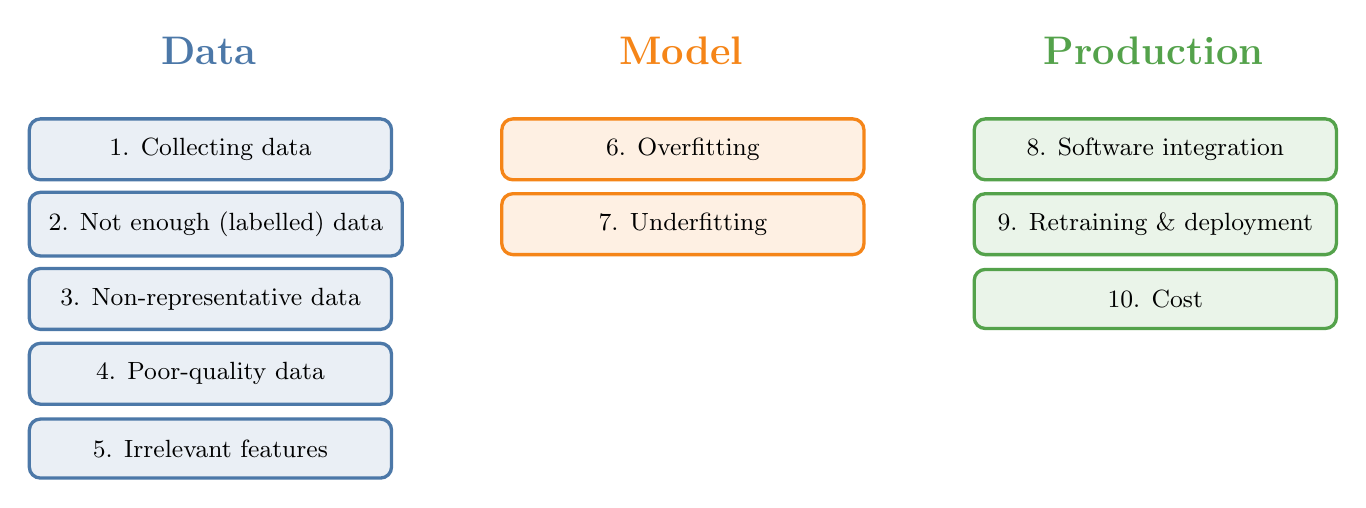
\begin{tikzpicture}
  \tikzset{item/.style={box=#1, minimum width=4.6cm, minimum height=0.75cm, font=\small, anchor=west}}
  \node[title, cblue] at (0,0.9) {Data};
  \foreach \t [count=\i] in {1. Collecting data, 2. Not enough (labelled) data, 3. Non-representative data, 4. Poor-quality data, 5. Irrelevant features}
    \node[item=cblue] at (-2.3,-\i*0.95+0.6) {\t};
  \node[title, corange] at (6.0,0.9) {Model};
  \foreach \t [count=\i] in {6. Overfitting, 7. Underfitting}
    \node[item=corange] at (3.7,-\i*0.95+0.6) {\t};
  \node[title, cgreen] at (12.0,0.9) {Production};
  \foreach \t [count=\i] in {8. Software integration, 9. Retraining \& deployment, 10. Cost}
    \node[item=cgreen] at (9.7,-\i*0.95+0.6) {\t};
\end{tikzpicture}
\end{document}
